\newpage

\setcounter{page}{1}
\setcounter{figure}{0}
\section{Uvod}% (fold)
\label{sec:Uvod}

% new opportunities to solve fundamental problems in computer vision. .
% The covered topics include preprocessing, object tracking and
% recognition, human activity analysis, hand gesture analysis, and
% indoor 3-D mapping. 

Pojava i dostupnost jeftinog i kvalitetnog 3D senzora Microsoft Kinect
kamere 2010. godine za igračku konzolu Xbox 360 uvelike je doprinjela
razvoju računalnog vida. Senzor u VGA rezoluciji frekvencijom od 30Hz
daje informacije o dubini i sliku u boji. Time omogućava da se na
prirodniji način pristupi rješavanju osnovnih problema računalnog vida.
Upravo to se i dogodilo te su znanstvenici, programeri i hakeri 
razvili upravljačke programa, alate i algoritme za korištenje Kineckt
senzora i sličnih uređaja za prikupljanje oblaka točaka. Većina
kreiranog softvera je objavljena pod slobodnim licencama koje
omogućavaju slobodu upotrebe programa u bilo koje svrhe, slobodu
proučavanja i primjenjivanja stečenog znanja, slobodu distribuiranja
kopija u cijelosti ili u dijelovima te slobodu mjenjanja, poboljšavanja
i distribuiranje derivacijskih programa. Upravo ti programi su postavili
temlje za ovaj diplomski rad.

Rad se sastoji iz tri dijela. Prvi dio odnosi se na pregled korištenih
tehnologija i algoritama. **Napisati jos koju recenicu o tehnologijama i
algoritmima**. Drugi dio je praktični dio i govori o izgradnji 3D modela
scene. Prvo je objašnjen postupak snimanja scene 3D kamerom i RGBDSlam
programom, a zatim je dan pregled izgradnje 3D modela scene mrežom
trokuta. Treći dio rada prikazuje rezultate snimanja i izrade te ispituje
funkcionalnost i kvalitetu postupka.


\newpage
\subsection{Zadatak diplomskog rada} % (fold)
\label{sub:Zadatak diplomskog rada}
\textbf{PRIVREMEN C/P opisa diplomskog} 
\\
Program RGBDSLAM raspoloživ u okviru programske biblioteke OpenSLAM
omogućava izgradnju 3D modela objekata i scena pomoću 3D kamere.
Razviti program za izgradnju 3D modela u obliku mreže trokuta koristeći
biblioteku PointCloud. Kombinacijom ova dva programa mogu se izgraditi
3D modeli objekata i scena snimljenih iz više pogleda. Zadatak je
ispitati funkcionalnost navedenog postupka kao i kvalitetu dobivenog
rezultata izgradnjom nekoliko 3D modela objekata i scena.

\begin{figure}[h]
\centering
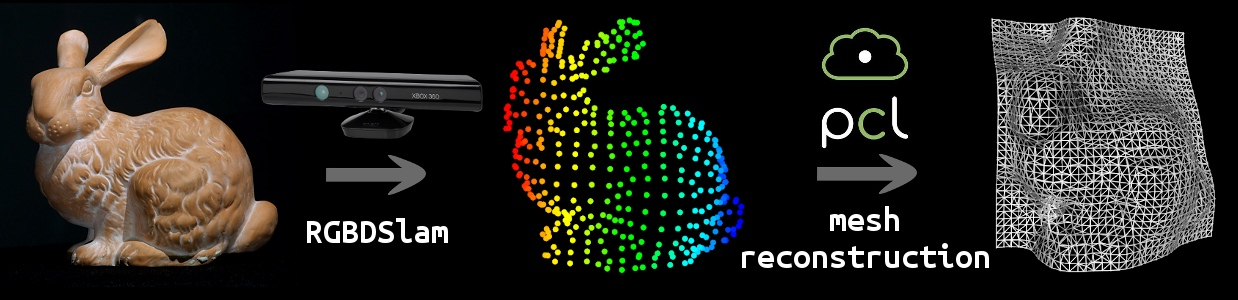
\includegraphics[scale=0.35]{figures/project-description.jpeg}
\caption[]{Grafički prikaz projekta upotrebom Standfordovog
zeca\footnotemark[1]}
\label{fig:project-description}
\end{figure}

\footnotetext[1]{%
Standford Bunny 3D model su originalno konstruirali 1994 Greg Turk i
Marc Levoy i od tada je postao najčešće upotrebljevani model za
testiranje tehnika u računalnoj grafici. \url{http://www.gvu.gatech.%
edu/people/faculty/greg.turk/bunny/bunny.html}
}

% subsection Zadatak diplomskog rada (end)
% section Uvod (end)
